%%%% Preamble
\documentclass[paper=a4,fontsize=11pt]{report}


%\begin{document}

%\begin{titlepage}
    
\newcommand{\HRule}{\rule{\linewidth}{0.5mm}} % Defines a new command for the horizontal lines, change thickness here
    
\center % Center everything on the page
     
%----------------------------------------------------------------------------------------
%	HEADING SECTIONS
%----------------------------------------------------------------------------------------
    
\textsc{\LARGE Instituto Tecnológico de Buenos Aires}\\[2cm] % Name of your university/college
\textsc{\Large Electronica III}\\[1.5cm] % Major heading such as course name
\textsc{\large Trabajo Práctico N° 2}\\[0.5cm] % Minor heading such as course title
    
%----------------------------------------------------------------------------------------
%	TITLE SECTION
%----------------------------------------------------------------------------------------
    
\HRule \\[0.5cm]
{ \huge \bfseries Trabajo Práctico de Laboratorio Nr. 2}\\[0.4cm] % Title of your document
\HRule \\[2cm]
     
%----------------------------------------------------------------------------------------
%	AUTHOR SECTION
%----------------------------------------------------------------------------------------
    
\begin{minipage}{0.4\textwidth}
\begin{flushleft} \large
\emph{Grupo 2:}\\		%names
[.3cm]
Victor \textsc{Oh}\\
Leg. ???\\ 
[.3cm]
Ian \textsc{Diaz}\\
Leg. ???\\ 
[.3cm]
Benjamín Carlos \textsc{Lin}\\
Leg. 57242 \\ 
[.3cm]
Malena \textsc{Muller}\\
Leg. ???\\ 
[.3cm]
\end{flushleft}
\end{minipage}
~
\begin{minipage}{0.4\textwidth}
\begin{flushright} \large
%\emph{Profesor:} \\
%[.3cm]
%Pablo  \textsc{Cossutta}\\ % Supervisor's Name
%Alejandra \textsc{Weill} \\% Supervisor's Name
%Matías  \textsc{Salvati} % Supervisor's Name
\end{flushright}
\end{minipage}\\[2cm]
    
%----------------------------------------------------------------------------------------
%	DATE SECTION
%----------------------------------------------------------------------------------------
    
\vfill
{\large Entregado: 17 de Octubre de 2018}\\[2cm]
    
\vfill 
    
\end{titlepage}
%
%\pagenumbering{roman}
%\tableofcontents
%\newpage
%\pagenumbering{arabic}
%
%Test Text

\section{\color{olive}Exercise 2: The Effect of the Noise Margin}

Having three different technology integrated circuits (74HC02, 74HCT02 and 74LS02), we compare the noise margin between them and analyze the possible results when loading them with each other as follows:

 \begin{figure}[h!]
        \centering
        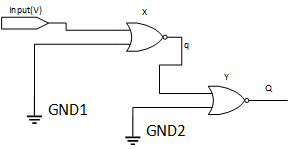
\includegraphics[scale=0.65]{../Exercise2/circuit2.png}
        \caption{\color{cyan}Logical circuit}
        \label{fig:ej2circ}
    \end{figure}

-Input(V): Input voltage; \\
-$X$: First component name; \\
-$Y$: Second component name; \\
-$q$: First result voltage; \\
-$Q$: Final result

	\subsection{\color{purple}Theoretically}
	
	 From the data-sheet of the components we obtain the following data when the power supply is $4.5V$ in the 74HC02 and 74HCT02 and around $5V$ for 74LS02:
	 
	 \begin{figure}[h!]
        \centering
        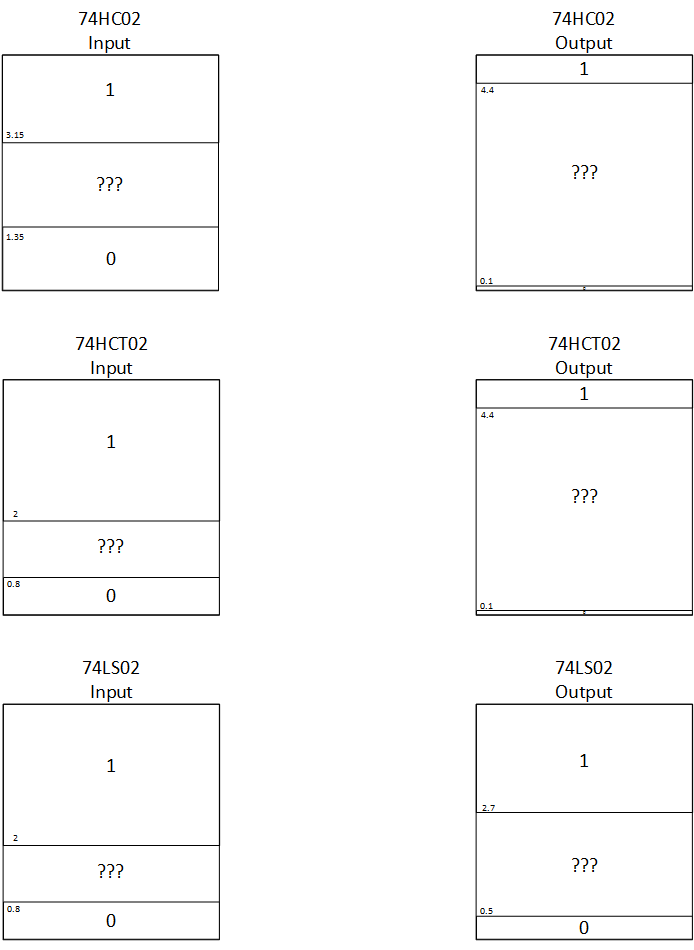
\includegraphics[scale=0.5]{../Exercise2/dataaa2.png}
        \caption{\color{cyan}Theoretical Noise Margin in Input and Output}
        \label{fig:ej2thnm}
    \end{figure}
    
    Within the mentioned values of power supply, the fanout of the components for 74HC02 and 74HCT02 is 20, with $I_l =\pm1{\mu}A$ and $I_o=-20{\mu}A$; and for 74LS02 is 80, with $I_l =0.1mA$ and $I_o=8mA$. As we load the components together, to avoid damaging the circuit, the maximum fanout allowed shall be the minimum of the components, this is to say 20 in this case when we load HC with LS or HCT with LS. 
    
    Connecting the circuit like in figure \ref{fig:ej2circ} being $X$ the second column and $Y$ the forth column, analysing the possible results would be:

	\begin{center}
	\hspace{2cm}\begin{table}[h!]
	\begin{tabular}{llllllllllllllllllll} 
	\cline{1-7}
	\multicolumn{1}{|c|}{\multirow{2}{*}{Input(V)}}                                & \multicolumn{2}{c|}{74HC02}                                                       & \multicolumn{1}{c|}{\multirow{2}{*}{q}}          & \multicolumn{2}{c|}{74LS02}                                          & \multicolumn{1}{c|}{\multirow{2}{*}{Q}}             \\ \cline{2-3} \cline{5-6}
	\multicolumn{1}{|c|}{}                                                 & \multicolumn{1}{c|}{Logic Input}        & \multicolumn{1}{c|}{Logic Output}       & \multicolumn{1}{c|}{}                            & \multicolumn{1}{c|}{Logic Input} & \multicolumn{1}{c|}{Logic Output} & \multicolumn{1}{c|}{}                               \\ \cline{1-7}
	\multicolumn{1}{|c|}{0\textless{}V\textless{}1.35}                     & \multicolumn{1}{c|}{0}                  & \multicolumn{1}{c|}{1}                  & \multicolumn{1}{c|}{4.4\textless{}V\textless{}5} & \multicolumn{1}{c|}{1}           & \multicolumn{1}{c|}{0}            & \multicolumn{1}{c|}{0\textless{}V\textless{}0.5}    \\ \cline{1-7}
	\multicolumn{1}{|c|}{\multirow{3}{*}{1.35\textless{}V\textless{}3.15}} & \multicolumn{1}{c|}{\multirow{3}{*}{?}} & \multicolumn{1}{c|}{\multirow{3}{*}{?}} & \multicolumn{1}{c|}{0\textless{}V\textless{}0.8} & \multicolumn{1}{c|}{0}           & \multicolumn{1}{c|}{1}            & \multicolumn{1}{c|}{2.7\textless{}V\textless{}5}    \\ \cline{4-7}
	\multicolumn{1}{|c|}{}                                                 & \multicolumn{1}{c|}{}                   & \multicolumn{1}{c|}{}                   & \multicolumn{1}{c|}{0.8\textless{}V\textless{}2} & \multicolumn{1}{c|}{?}           & \multicolumn{1}{c|}{?}            & \multicolumn{1}{c|}{0.5\textless{}V\textless{}2.7}  \\ \cline{4-7}
	\multicolumn{1}{|c|}{}                                                 & \multicolumn{1}{c|}{}                   & \multicolumn{1}{c|}{}                   & \multicolumn{1}{c|}{2\textless{}V\textless{}4.4} & \multicolumn{1}{c|}{1}           & \multicolumn{1}{c|}{0}            & \multicolumn{1}{c|}{0\textless{}V\textless{}0.5}    \\ \cline{1-7}
	\multicolumn{1}{|c|}{3.15\textless{}V\textless{}5}                     & \multicolumn{1}{c|}{1}                  & \multicolumn{1}{c|}{0}                  & \multicolumn{1}{c|}{0\textless{}V\textless{}0.1} & \multicolumn{1}{c|}{0}           & \multicolumn{1}{c|}{1}            & \multicolumn{1}{c|}{2.7\textless{}V\textless{}5}\\ \cline{1-7}
	\end{tabular}
	\caption{\color{cyan}74HC02 load to 74LS02}
	\label{fig:ej2thhctols}
	\end{table}
	\end{center}
	
	\begin{center}
	\hspace{1cm}\begin{table}[h!]
	\begin{tabular}{llllllllllllllllllll}
	\cline{1-7}
	\multicolumn{1}{|c|}{\multirow{2}{*}{Input(V)}} & \multicolumn{2}{c|}{74LS02} & \multicolumn{1}{c|}{\multirow{2}{*}{q}} & \multicolumn{2}{c|}{74HC02} & \multicolumn{1}{c|}{\multirow{2}{*}{Q}}  \\ \cline{2-3} \cline{5-6}
	\multicolumn{1}{|c|}{} & \multicolumn{1}{c|}{Logic Input} & \multicolumn{1}{c|}{Logic Output} & \multicolumn{1}{c|}{} & \multicolumn{1}{c|}{Logic Input} & \multicolumn{1}{c|}{Logic Output} & \multicolumn{1}{c|}{}  \\ \cline{1-7}
	\multicolumn{1}{|c|}{\multirow{2}{*}{0\textless{}V\textless{}0.8}} & \multicolumn{1}{c|}{\multirow{2}{*}{0}} & \multicolumn{1}{c|}{\multirow{2}{*}{1}} & \multicolumn{1}{c|}{2.7\textless{}V\textless{}3.15} & \multicolumn{1}{c|}{?} & \multicolumn{1}{c|}{?} & \multicolumn{1}{c|}{0.1\textless{}V\textless{}4.4}  \\ \cline{4-7}
	\multicolumn{1}{|c|}{} & \multicolumn{1}{c|}{} & \multicolumn{1}{c|}{} & \multicolumn{1}{c|}{3.15\textless{}V\textless{}5} & \multicolumn{1}{c|}{1} & \multicolumn{1}{c|}{0} & \multicolumn{1}{c|}{0\textless{}V\textless{}0.1}  \\ \cline{1-7}
	\multicolumn{1}{|c|}{\multirow{2}{*}{0.8\textless{}V\textless{}2}} & \multicolumn{1}{c|}{\multirow{2}{*}{?}} & \multicolumn{1}{c|}{\multirow{2}{*}{?}} & \multicolumn{1}{c|}{0.5\textless{}V\textless{}1.35} & \multicolumn{1}{c|}{0} & \multicolumn{1}{c|}{1} & \multicolumn{1}{c|}{4.4\textless{}V\textless{}5}  \\ \cline{4-7}
	\multicolumn{1}{|c|}{} & \multicolumn{1}{c|}{} & \multicolumn{1}{c|}{} & \multicolumn{1}{c|}{1.35\textless{}V\textless{}2.7} & \multicolumn{1}{c|}{?} & \multicolumn{1}{c|}{?} & \multicolumn{1}{c|}{0.1\textless{}V\textless{}4.4}  \\ \cline{1-7}
	\multicolumn{1}{|c|}{2\textless{}V\textless{}5} & \multicolumn{1}{c|}{1} & \multicolumn{1}{c|}{0} & \multicolumn{1}{c|}{0\textless{}V\textless{}0.5} & \multicolumn{1}{c|}{0} & \multicolumn{1}{c|}{1} & \multicolumn{1}{c|}{4.4\textless{}V\textless{}5}\\ \cline{1-7}
	\end{tabular}
	\caption{\color{cyan}74LS02 load to 74HC02}
	\label{fig:ej2thlstohc}
	\end{table}
	\end{center}
	
	\begin{center}
	\hspace{1cm}\begin{table}[h!]
	\begin{tabular}{llllllllllllllllllll}
	\cline{1-7}
	\multicolumn{1}{|c|}{\multirow{2}{*}{Input(V)}} & \multicolumn{2}{c|}{74LS02} & \multicolumn{1}{c|}{\multirow{2}{*}{q}} & \multicolumn{2}{c|}{74HCT02} & \multicolumn{1}{c|}{\multirow{2}{*}{Q}}  \\ \cline{2-3} \cline{5-6}
	\multicolumn{1}{|c|}{} & \multicolumn{1}{c|}{Logic Input} & \multicolumn{1}{c|}{Logic Output} & \multicolumn{1}{c|}{} & \multicolumn{1}{c|}{Logic Input} & \multicolumn{1}{c|}{Logic Output} & \multicolumn{1}{c|}{}  \\ \cline{1-7}
	\multicolumn{1}{|c|}{0\textless{}V\textless{}0.8} & \multicolumn{1}{c|}{0} & \multicolumn{1}{c|}{1} & \multicolumn{1}{c|}{2.7\textless{}V\textless{}5} & \multicolumn{1}{c|}{1} & \multicolumn{1}{c|}{0} & \multicolumn{1}{c|}{4.4\textless{}V\textless{}5}  \\ \cline{1-7}
	\multicolumn{1}{|c|}{\multirow{3}{*}{0.8\textless{}V\textless{}2}} & \multicolumn{1}{c|}{\multirow{3}{*}{?}} & \multicolumn{1}{c|}{\multirow{3}{*}{?}} & \multicolumn{1}{c|}{0.5\textless{}V\textless{}0.8} & \multicolumn{1}{c|}{0} & \multicolumn{1}{c|}{1} & \multicolumn{1}{c|}{4.4\textless{}V\textless{}5}  \\ \cline{4-7}
	\multicolumn{1}{|c|}{} & \multicolumn{1}{c|}{} & \multicolumn{1}{c|}{} & \multicolumn{1}{c|}{0.8\textless{}V\textless{}2} & \multicolumn{1}{c|}{?} & \multicolumn{1}{c|}{?} & \multicolumn{1}{c|}{0.1\textless{}V\textless{}4.4}  \\ \cline{4-7}
	\multicolumn{1}{|c|}{} & \multicolumn{1}{c|}{} & \multicolumn{1}{c|}{} & \multicolumn{1}{c|}{2\textless{}V\textless{}2.7} & \multicolumn{1}{c|}{1} & \multicolumn{1}{c|}{0} & \multicolumn{1}{c|}{0\textless{}V\textless{}0.1}  \\ \cline{1-7}
	\multicolumn{1}{|c|}{2\textless{}V\textless{}5} & \multicolumn{1}{c|}{1} & \multicolumn{1}{c|}{0} & \multicolumn{1}{c|}{0\textless{}V\textless{}0.5} & \multicolumn{1}{c|}{0} & \multicolumn{1}{c|}{1} & \multicolumn{1}{c|}{4.4\textless{}V\textless{}5}\\ \cline{1-7}
	\end{tabular}
	\caption{\color{cyan}74LS02 load to 74HCT02}
	\label{fig:ej2thlstohct}
	\end{table}
	\end{center}
	
	\begin{center}
	\hspace{1cm}\begin{table}[h!]
	\begin{tabular}{llllllllllllllllllll}
	\cline{1-7}
	\multicolumn{1}{|c|}{\multirow{2}{*}{Input(V)}} & \multicolumn{2}{c|}{74HCT02} & \multicolumn{1}{c|}{\multirow{2}{*}{q}} & \multicolumn{2}{c|}{74LS02} & \multicolumn{1}{c|}{\multirow{2}{*}{Q}}  \\ \cline{2-3} \cline{5-6}
	\multicolumn{1}{|c|}{} & \multicolumn{1}{c|}{Logic Input} & \multicolumn{1}{c|}{Logic Output} & \multicolumn{1}{c|}{} & \multicolumn{1}{c|}{Logic Input} & \multicolumn{1}{c|}{Logic Output} & \multicolumn{1}{c|}{}  \\ \cline{1-7}
	\multicolumn{1}{|c|}{0\textless{}V\textless{}0.8} & \multicolumn{1}{c|}{0} & \multicolumn{1}{c|}{1} & \multicolumn{1}{c|}{4.4\textless{}V\textless{}5} & \multicolumn{1}{c|}{1} & \multicolumn{1}{c|}{0} & \multicolumn{1}{c|}{0\textless{}V\textless{}0.5}  \\ \cline{1-7}
	\multicolumn{1}{|c|}{\multirow{3}{*}{0.8\textless{}V\textless{}2}} & \multicolumn{1}{c|}{\multirow{3}{*}{?}} & \multicolumn{1}{c|}{\multirow{3}{*}{?}} & \multicolumn{1}{c|}{0.1\textless{}V\textless{}0.8} & \multicolumn{1}{c|}{0} & \multicolumn{1}{c|}{1} & \multicolumn{1}{c|}{2.7\textless{}V\textless{}5}  \\ \cline{4-7}
	\multicolumn{1}{|c|}{} & \multicolumn{1}{c|}{} & \multicolumn{1}{c|}{} & \multicolumn{1}{c|}{0.8\textless{}V\textless{}2} & \multicolumn{1}{c|}{?} & \multicolumn{1}{c|}{?} & \multicolumn{1}{c|}{0.5\textless{}V\textless{}2.7}  \\ \cline{4-7}
	\multicolumn{1}{|c|}{} & \multicolumn{1}{c|}{} & \multicolumn{1}{c|}{} & \multicolumn{1}{c|}{2\textless{}V\textless{}4.4} & \multicolumn{1}{c|}{1} & \multicolumn{1}{c|}{0} & \multicolumn{1}{c|}{0\textless{}V\textless{}0.5}  \\ \cline{1-7}
	\multicolumn{1}{|c|}{2\textless{}V\textless{}5} & \multicolumn{1}{c|}{1} & \multicolumn{1}{c|}{0} & \multicolumn{1}{c|}{0\textless{}V\textless{}0.1} & \multicolumn{1}{c|}{0} & \multicolumn{1}{c|}{1} & \multicolumn{1}{c|}{2.7\textless{}V\textless{}5}\\ \cline{1-7}
	\end{tabular}
	\caption{\color{cyan}74HCT02 load to 74LS02}
	\label{fig:ej2thhcttols}
	\end{table}
	\end{center}
	
	\pagebreak
	
	Therefore, we expect, when loading the components, irregularities in the Q output value when the input value isn't the recommended in the data-sheet. 

	\subsection{\color{purple}Experimentally}
	
	Building the circuit in the figure \ref{fig:ej2circ}, with a squeare 0-5V signal, the measured results are:
	
	\begin{figure}[h!]
        \centering
        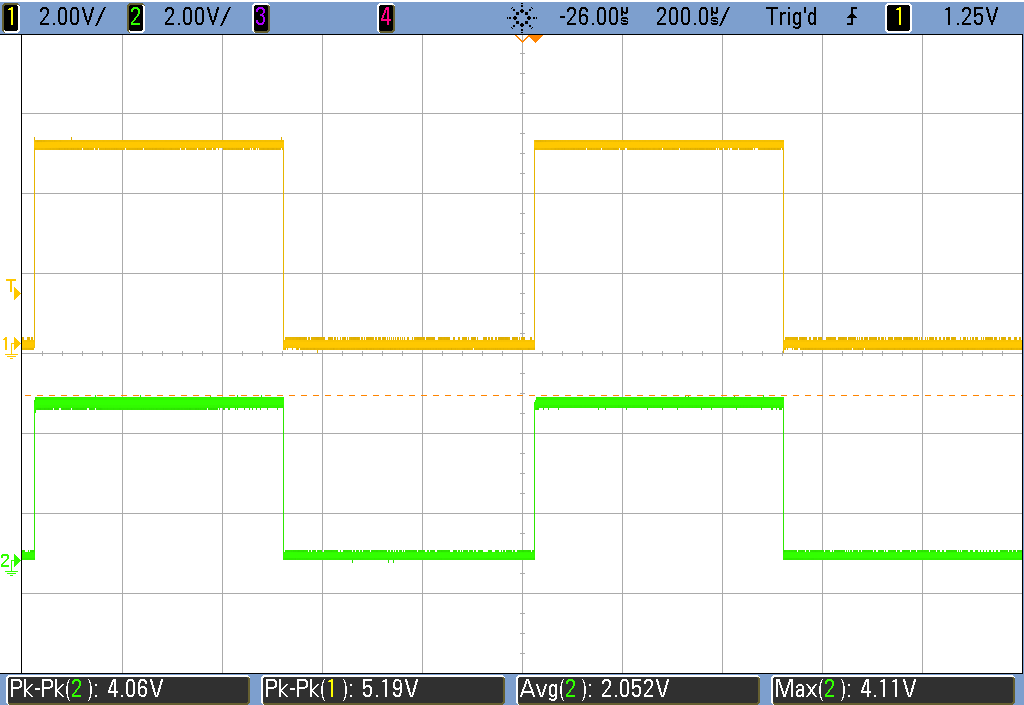
\includegraphics[scale=0.19]{../Exercise2/HC-LS-5V.png}\hspace{1cm}
%        \includegraphics[scale=0.19]{HC-LS-2V.png}\\
        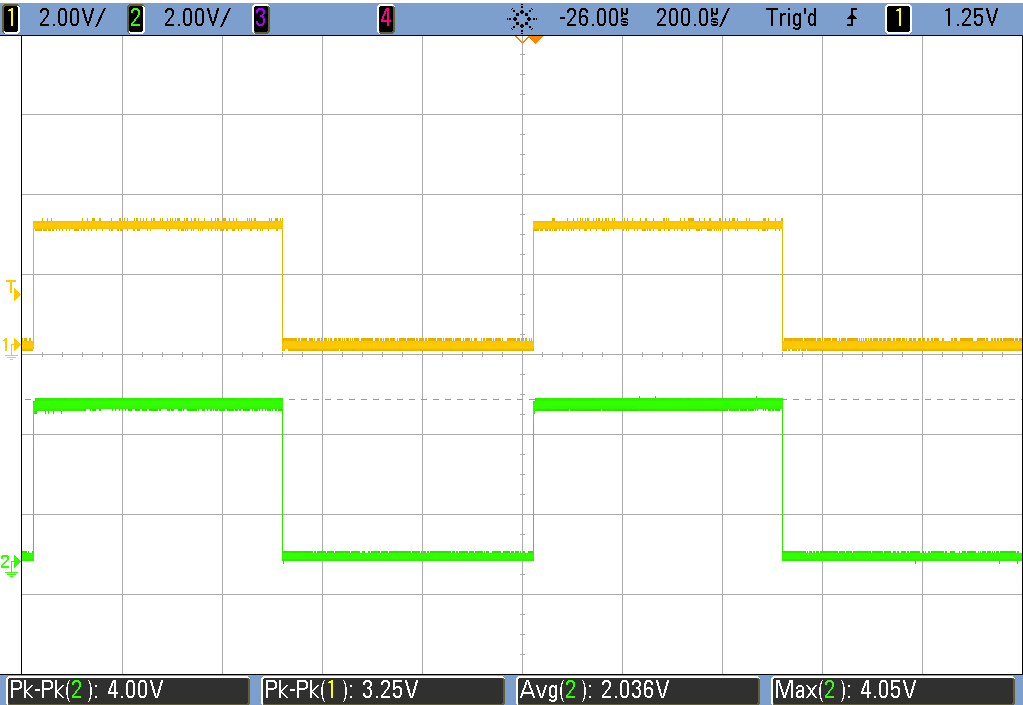
\includegraphics[scale=0.19]{../Exercise2/HC-LS-3V.png}\\
		\vspace{0.2cm}
%		\hspace{0.9cm}
	   \includegraphics[scale=0.19]{../Exercise2/HC-LS-2V.png}\hspace{1cm} 
        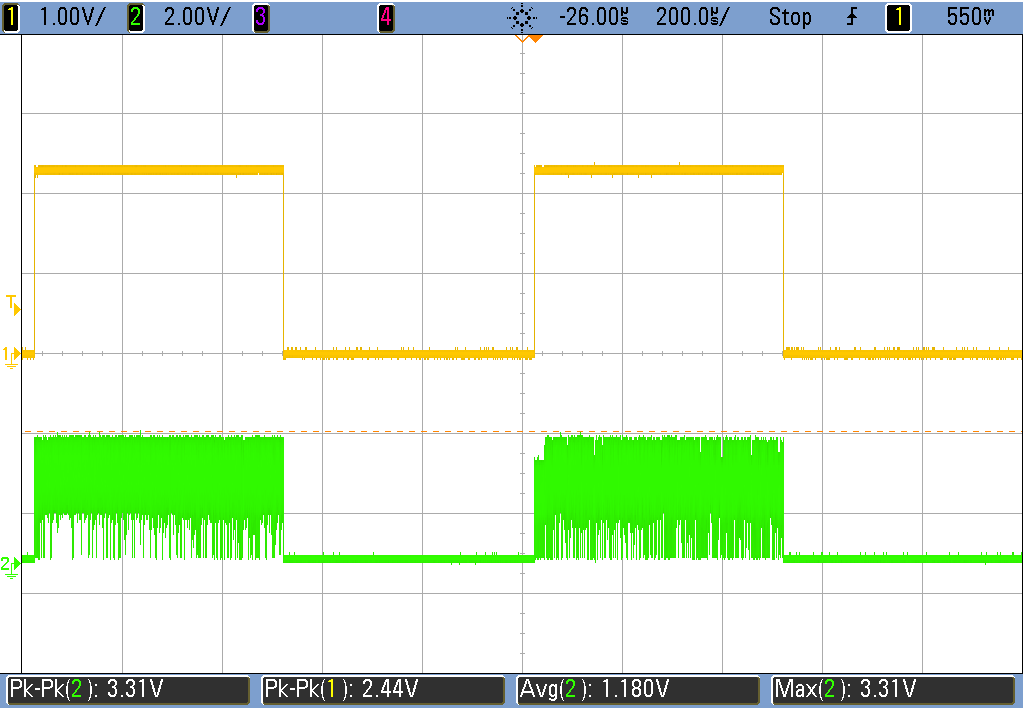
\includegraphics[scale=0.19]{../Exercise2/HC-LS-2p3V.png}
        \caption{\color{cyan}74HC02 load to 74LS02}
        \label{fig:ej2exhctols}
    \end{figure}
    
    \begin{figure}[h!]
        \centering
        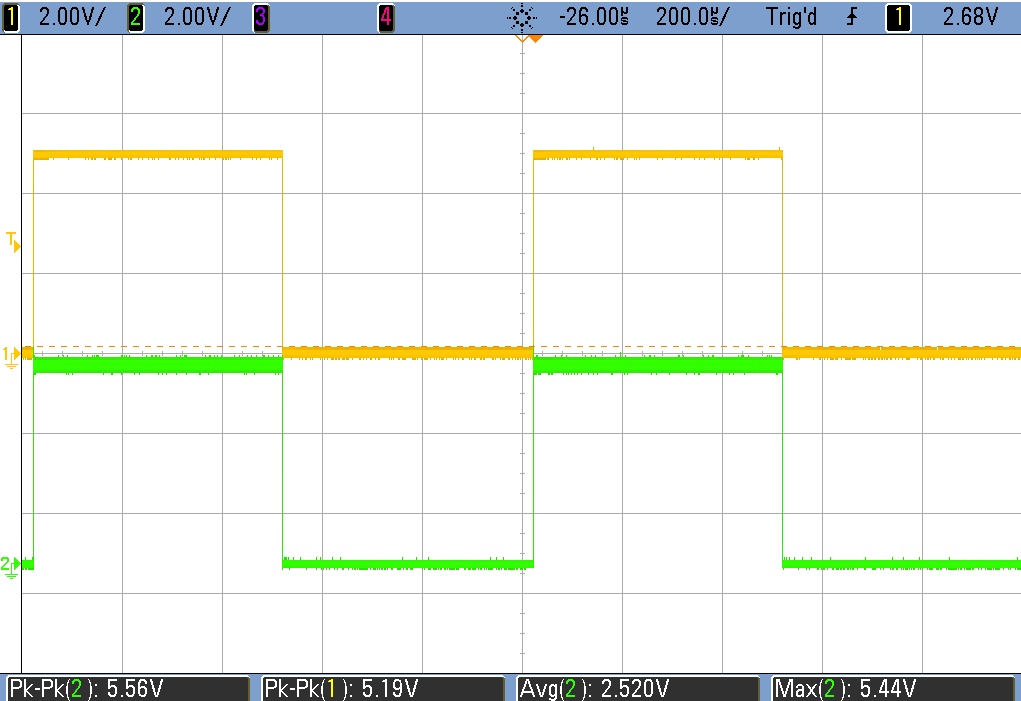
\includegraphics[scale=0.19]{../Exercise2/LS-HC-5V.png}\hspace{1cm}
        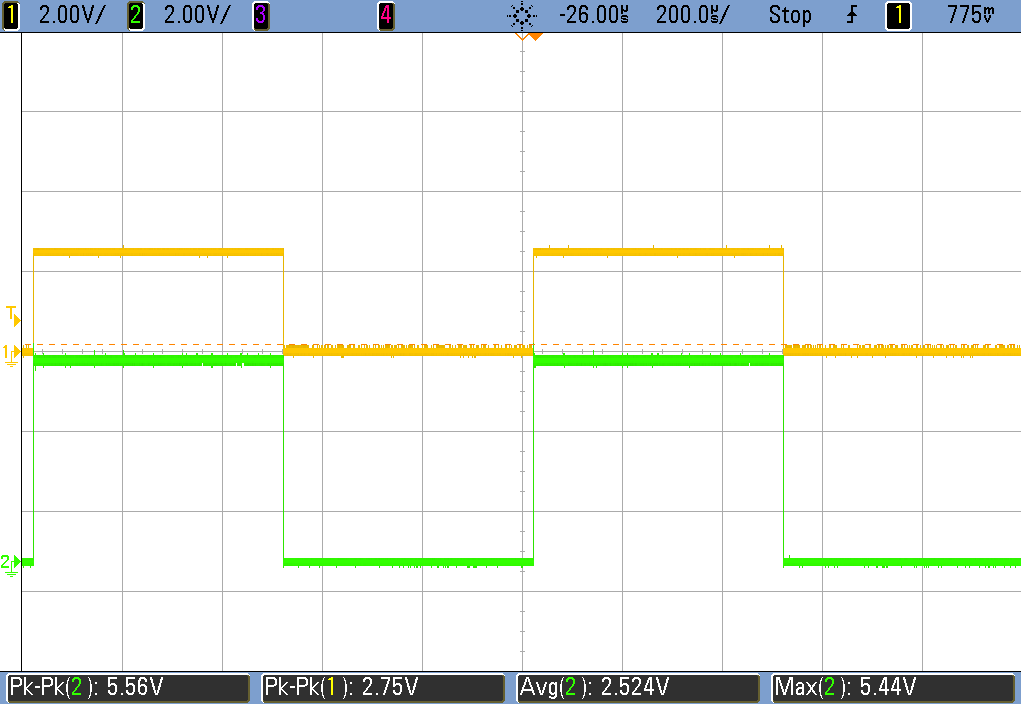
\includegraphics[scale=0.19]{../Exercise2/LS-HC-3V.png}\\
		\vspace{0.2cm}
%		\hspace{0cm}
        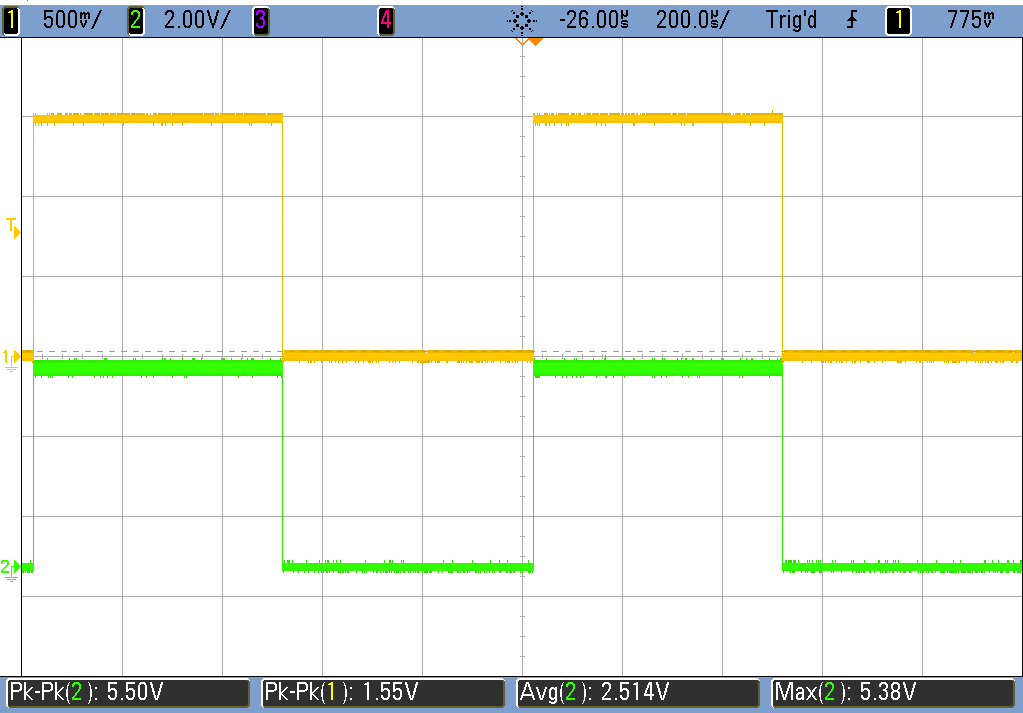
\includegraphics[scale=0.19]{../Exercise2/LS-HC-1p5V.png}\hspace{1cm}
         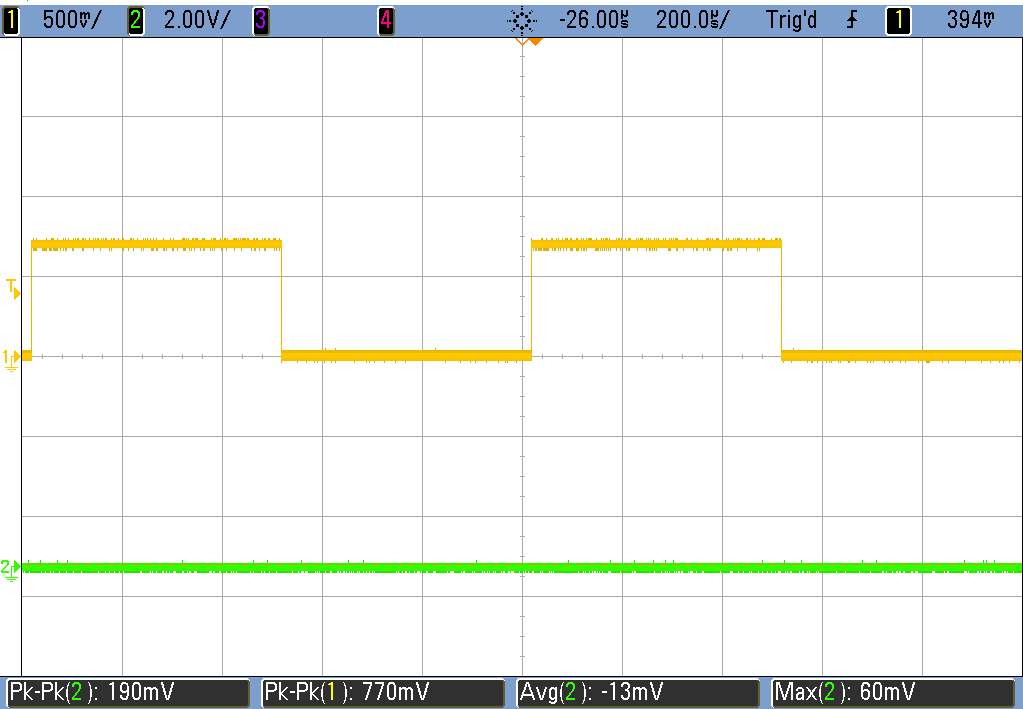
\includegraphics[scale=0.19]{../Exercise2/LS-HC-0p7V.png}\\
        \vspace{0.2cm}
%		\hspace{0.9cm}
        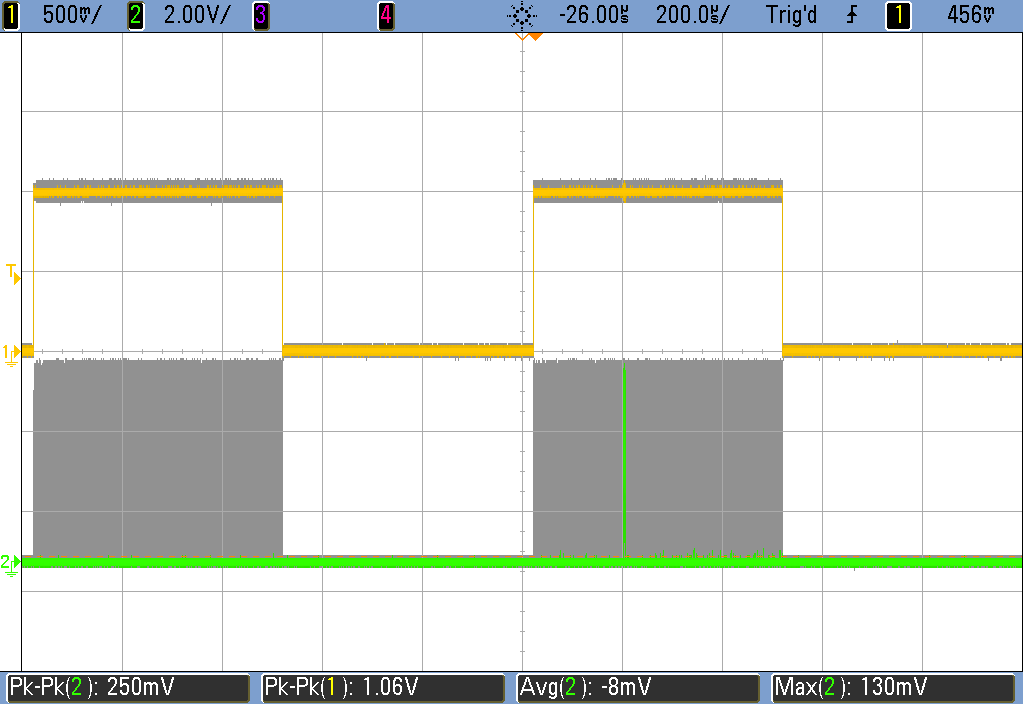
\includegraphics[scale=0.19]{../Exercise2/LS-HC-1V.png}
        \caption{\color{cyan}74LS02 load to 74HC02}
        \label{fig:ej2exlstohc}
    \end{figure}
    
%    \pagebreak
    \begin{figure}[h!]
        \centering
        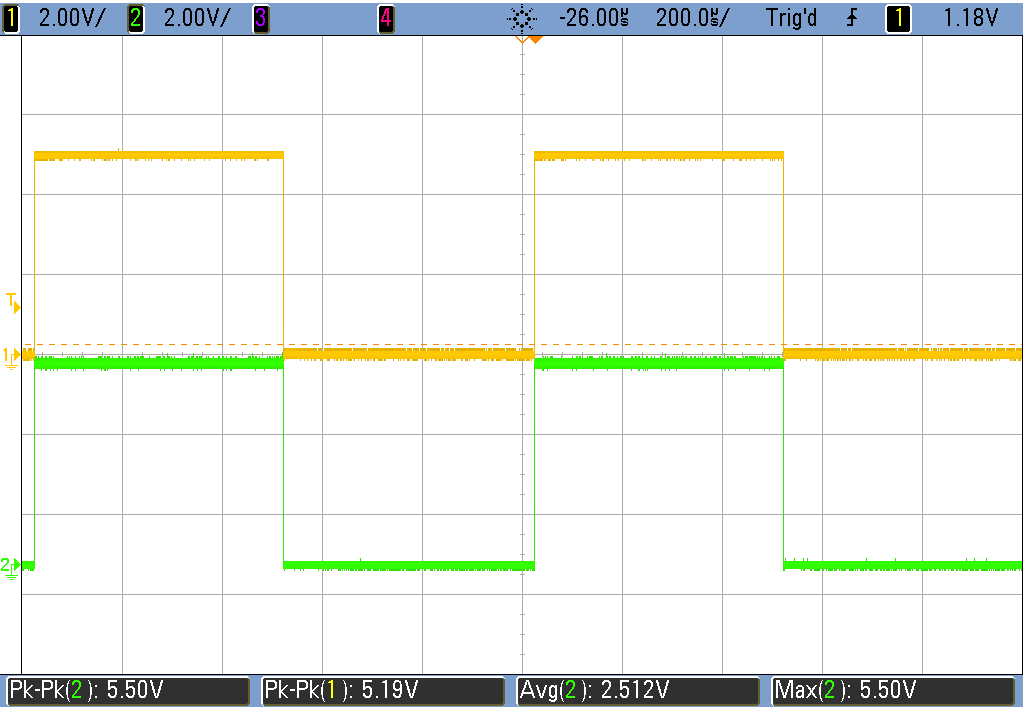
\includegraphics[scale=0.19]{../Exercise2/LS-HCT-5V.png}\hspace{1cm}
        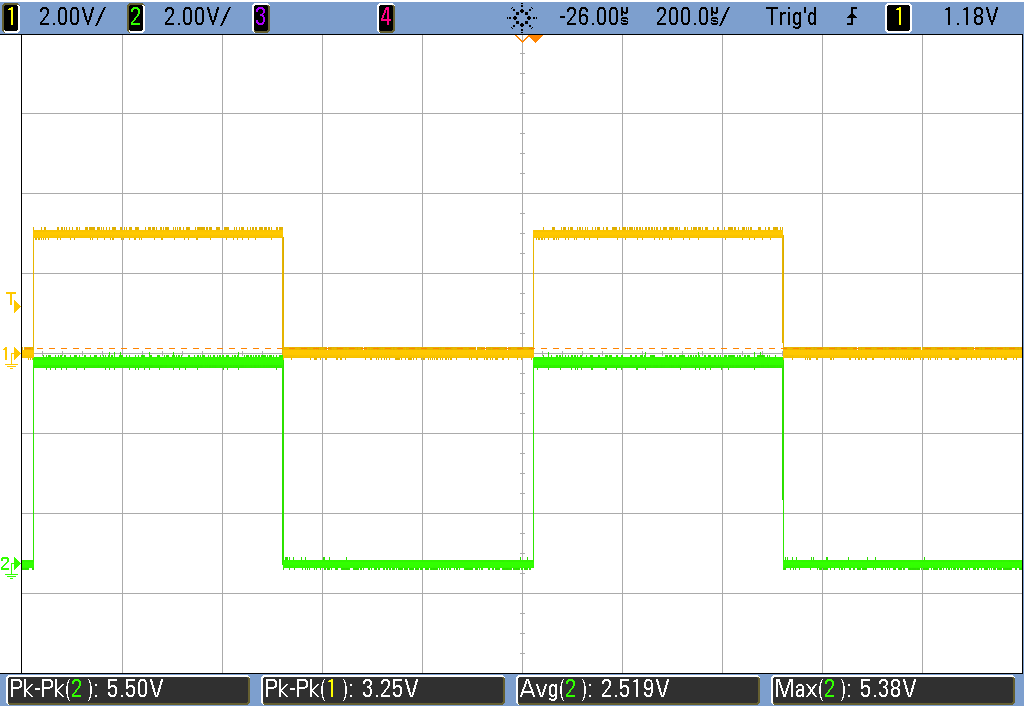
\includegraphics[scale=0.19]{../Exercise2/LS-HCT-3V.png}\\
		\vspace{0.2cm}
%		\hspace{0cm}
        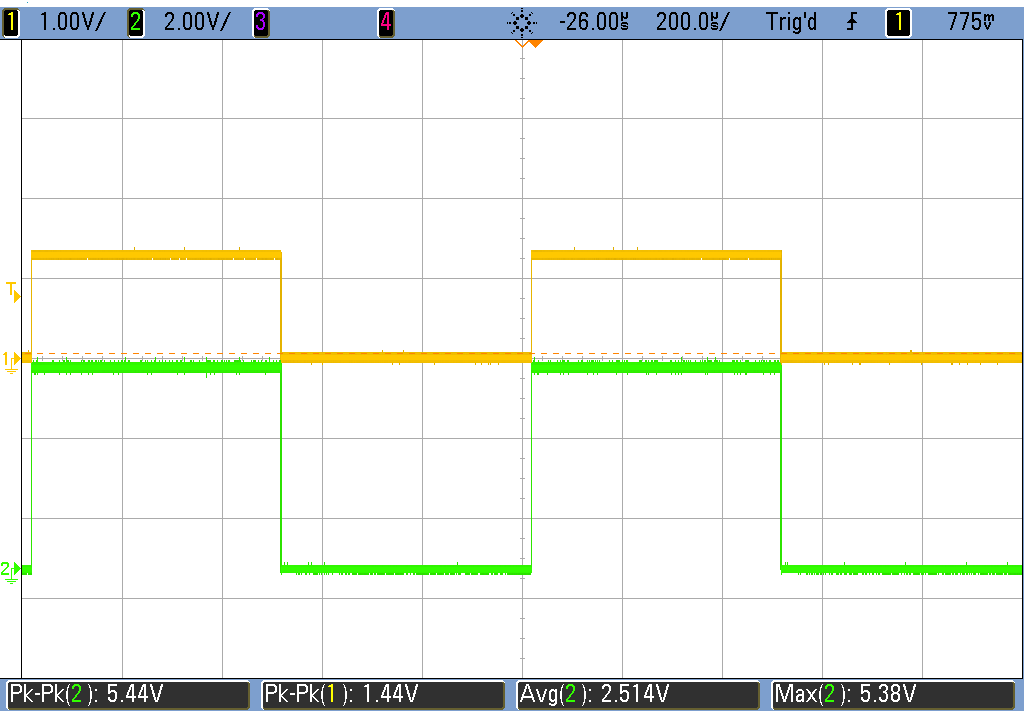
\includegraphics[scale=0.19]{../Exercise2/LS-HCT-1p5V.png}\hspace{1cm}
        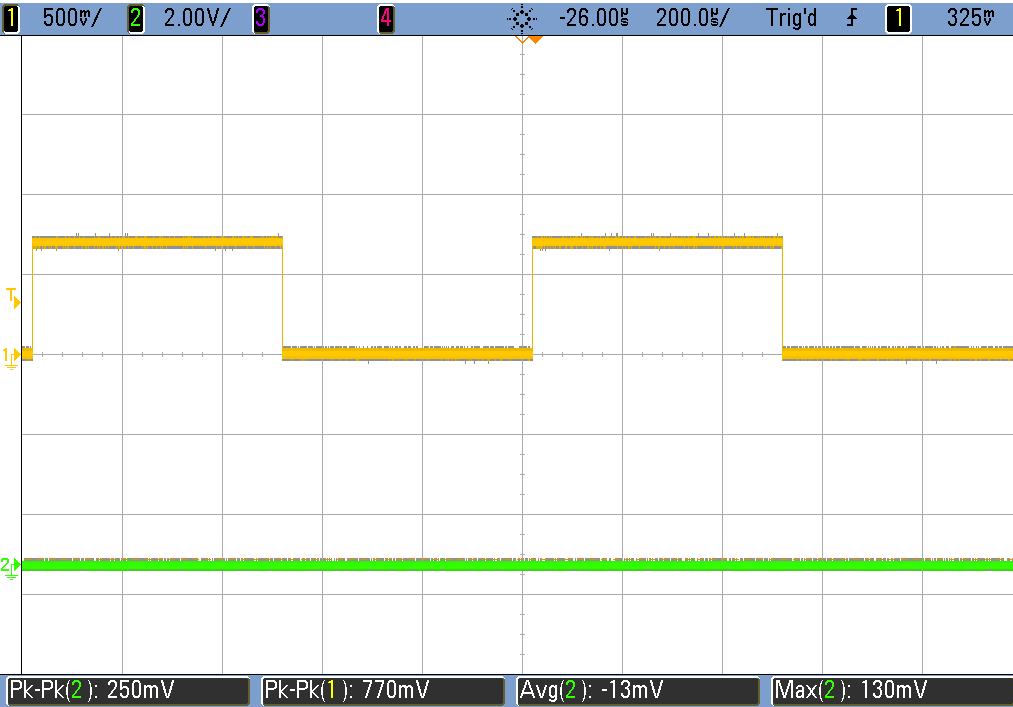
\includegraphics[scale=0.19]{../Exercise2/LS-HCT-0p7V.png}\\
        \vspace{0.2cm}
%		\hspace{0.9cm}
        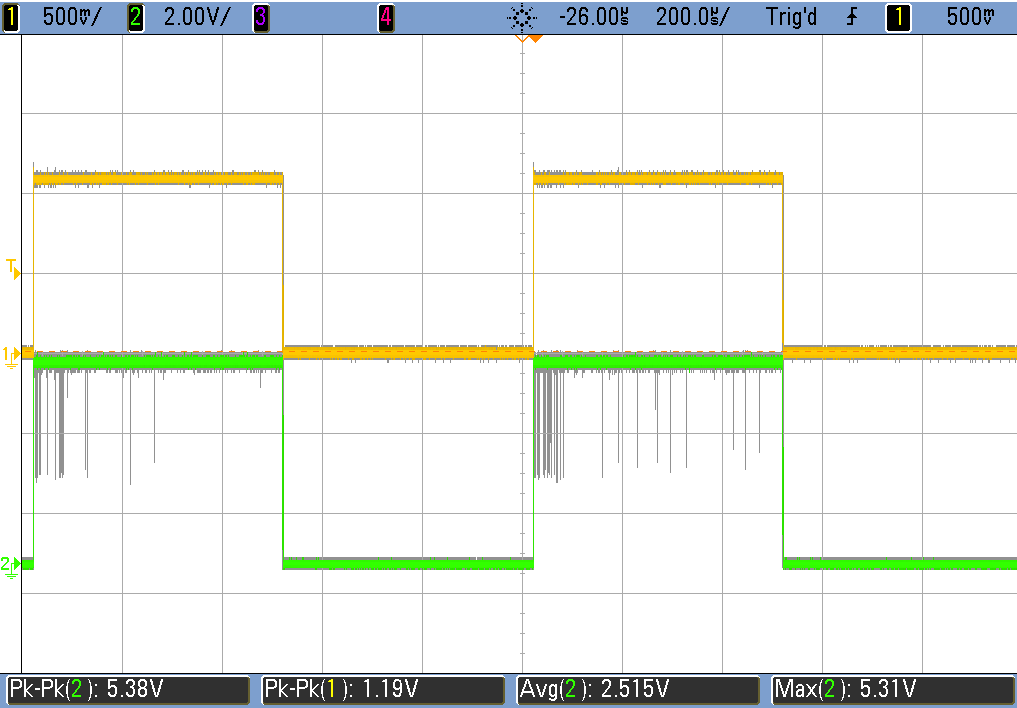
\includegraphics[scale=0.19]{../Exercise2/LS-HCT-1p1V.png}
        \caption{\color{cyan}74LS02 load to 74HCT02}
        \label{fig:ej2exlstohct}
    \end{figure}

    \begin{figure}[h!]
        \centering
        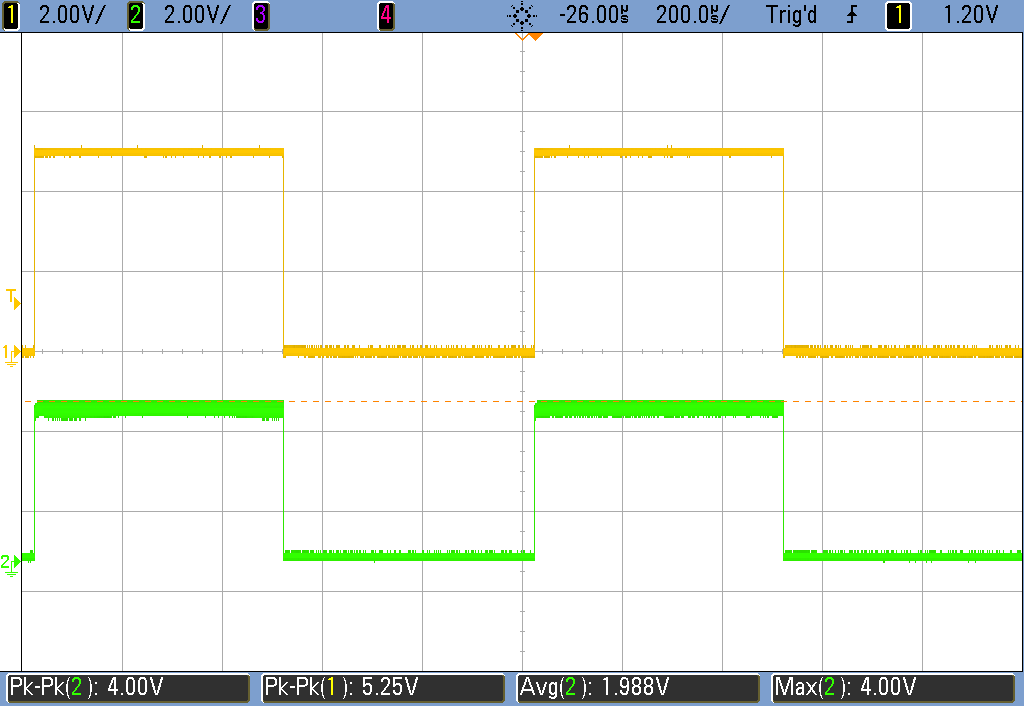
\includegraphics[scale=0.18]{../Exercise2/HCT-LS-5V.png}\hspace{1cm}
        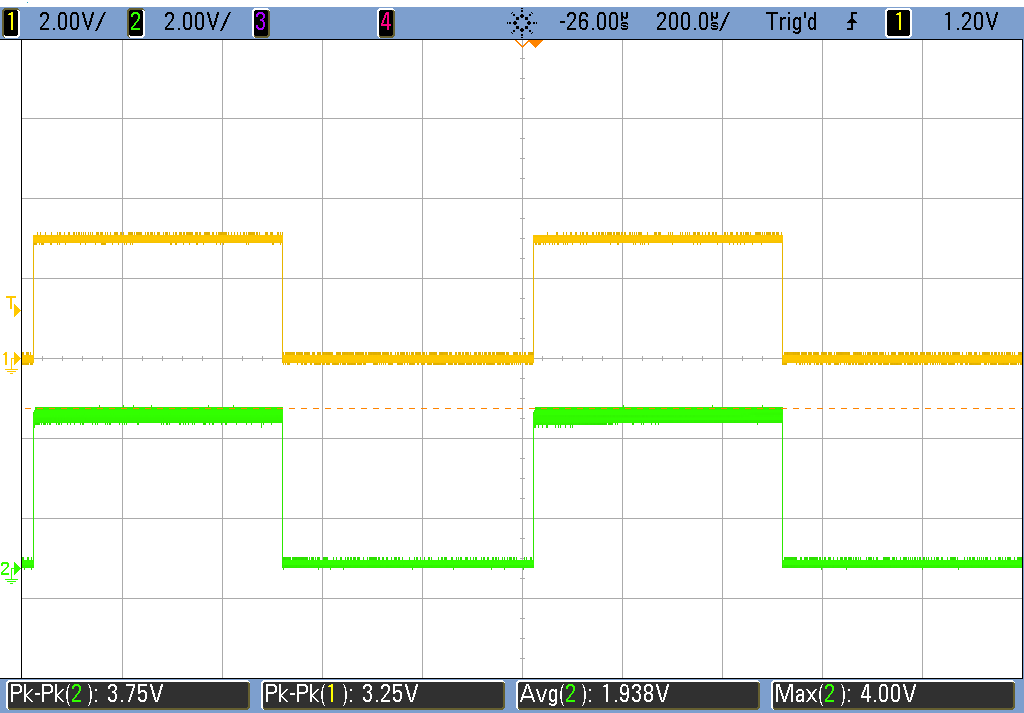
\includegraphics[scale=0.18]{../Exercise2/HCT-LS-3V.png}\\
		\vspace{0.2cm}
%		\hspace{0.9cm}
	   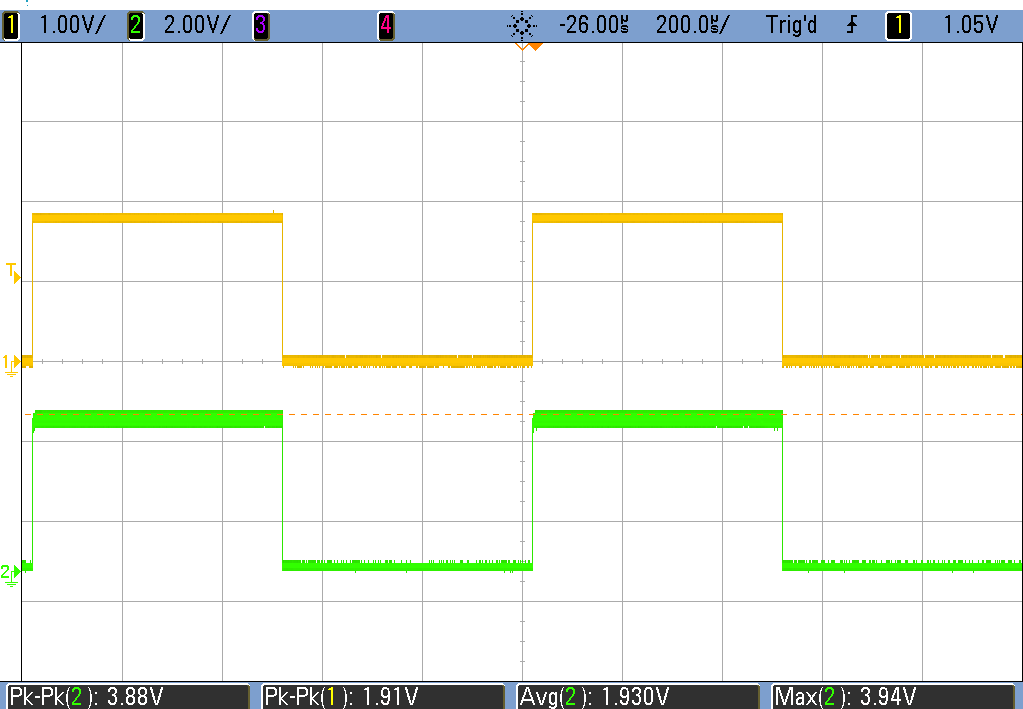
\includegraphics[scale=0.18]{../Exercise2/HCT-LS-1p8V.png}\hspace{1cm}
	   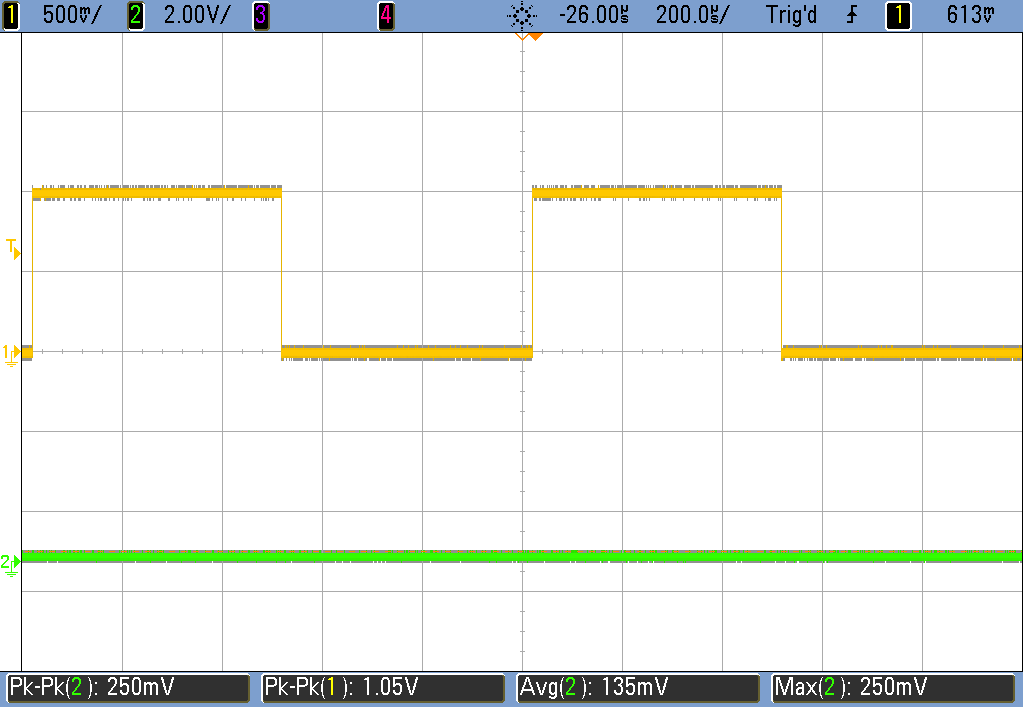
\includegraphics[scale=0.18]{../Exercise2/HCT-LS-1V.png}\\
	   \vspace{0.2cm}
%		\hspace{0cm}
%        \hspace{1cm}
        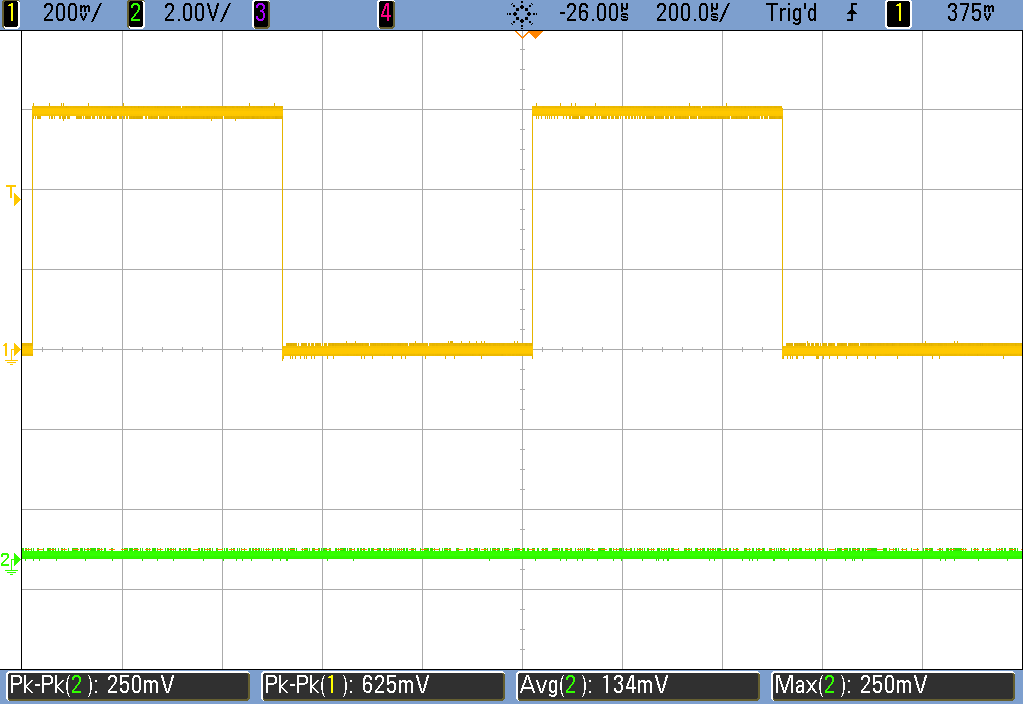
\includegraphics[scale=0.18]{../Exercise2/HCT-LS-0p6V.png}\hspace{1cm}
        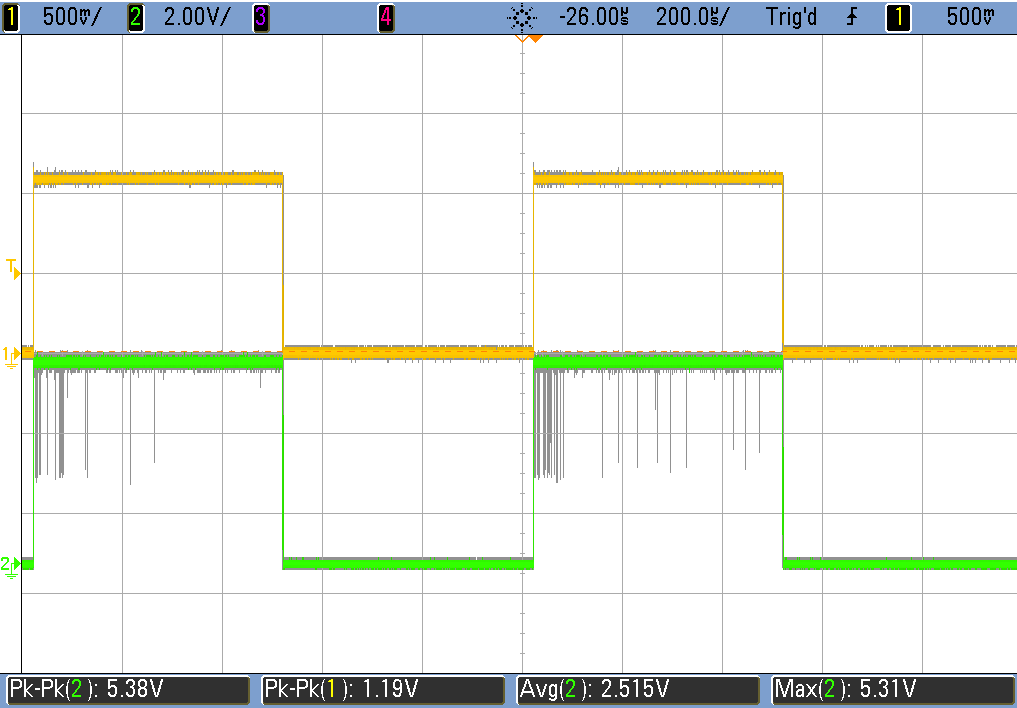
\includegraphics[scale=0.18]{../Exercise2/LS-HCT-1p1V.png}
        \caption{\color{cyan}74HCT02 load to 74LS02}
        \label{fig:ej2exhcttols}
    \end{figure}
    
    \pagebreak

	Analysing the results in $Q$ it is clear that the irregularities are odd to find, this could be because the manufacturer always leaves a bigger margin to avoid conflicts within each component. Moreover, as mentioned in the theoretical table when the input voltage isn't a logical input, the supply voltage is in the prohibited zone because the circuit cannot decide if the value of the voltage is low or high, the output value $q$ could mean something in the second component leading to misunderstandings or errors in the logical function. On the other hand, we can notice that using the HCT with the LS integrated circuits, their irregularity is lower in amplitude and not so defined as HC with LS, because their input noise margins are similar. 

%\end{document}